\section{Versuchsdurchführung und Auswertung}

\subsection{Verbleibende Aktivität}

Die 22-Na Probe wurde laut Beschriftung am Versuchsaufbau am 29.09.1993 eingesetzt. Sie hatte damals eine Aktivität von $A_{93} = 3,7\e{6} Bq$ und die Halbwertszeit wird mit $t_{1/2} = 2,6 a$ angegeben. Somit ergibt sich für die Restaktivität:
\begin{eqnarray*}
 A(t) = & A_{93} * e^{-\frac{\ln 2}{t_{1/2}} t} \\
      \approx & 3,61\e{4} Bq
\end{eqnarray*}
Die Messungen in der Staatsexamensarbeit wurden bei $A_{St} = 0,15 mCurie = 5,55\e{6} Bq$ durchgeführt. Wir erwarten also dass die Rate der Ereignisse im Experiment bei uns in etwa zwei Größenordnungen kleiner sein wird. Für die statistische Genauigkeit der Messungen ist dies nicht von Vorteil.

\subsection{Szintillatorspektren}
Wir haben das Spektrum des 22Na mit jedem der drei Szintillatoren aufgenommen (siehe Abb. \ref{22na-schrottspektrum}). Dazu haben wir je einen direkt an den Multi Channel Analysator (MCA) angeschlossen und 20 min gemessen.

\begin{figure}
 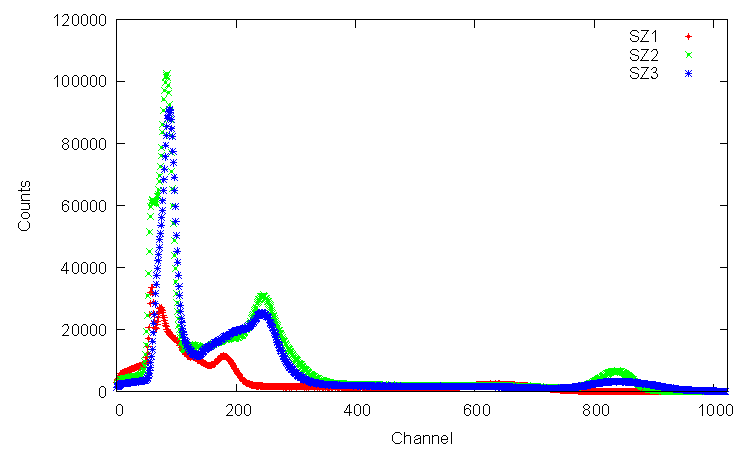
\includegraphics[width=\textwidth]{Graphen/Na-Spektren/na-spektren-1.pdf}
 \caption{Spektrum des 22Na Zerfalls, aufgenommen mit drei ungefilterten Szintilatoren}
 \label{22na-schrottspektrum}
\end{figure}

Dabei haben wir folgende Verstärkungen eingestellt:
SZ1: 8,13
SZ2: 5,00
SZ3: 10,00

Bei dem kleineren Peak mit hoher Energie (ca. Channel 850) handelt es sich nicht, wie von uns zuerst vermutet, um die 1270keV Gamma-Quanten des 22Ka-Zerfalls. Vielmehr scheint es sich um einen von der Elektronik erzeugten Störeffekt zu handeln. Der Peak mit der zweithöchsten Energie (Ch.250 bzw. 180) ist dann der eigentliche 1270keV Peak. Die 511keV des Zwei-Photonen-Zerfalls, die Photonen des 3er-Zerfalls und die Bremsstrahlung sind nur schlecht aufgelöst (SZ1 und SZ2) bzw. gar nicht unterscheidbar (SZ3).

Da wir außerdem beim Zuschalten des Single Channel Analysators (SCA) eine Verschiebung des Spektrums beobachteten, haben wir die Energiekalibration dann mit diesem durchgeführt.
\begin{figure}
 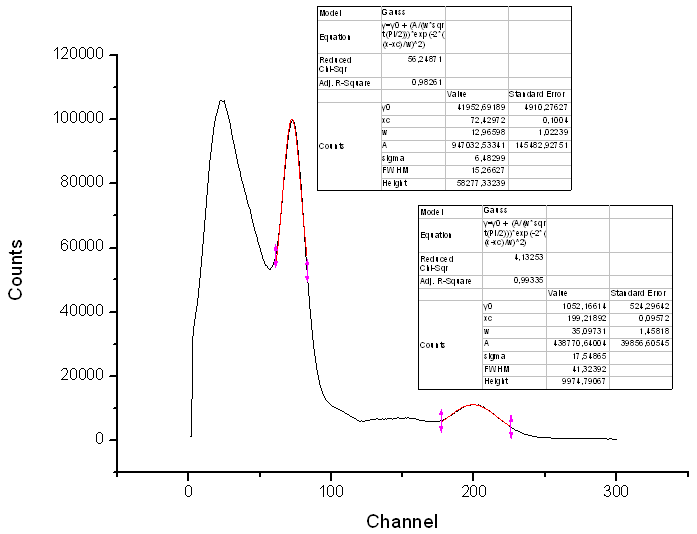
\includegraphics[width=\textwidth]{Graphen/SZ1.png}
 \caption{22Na Spektrum mit SZ1}
\end{figure}

\begin{figure}
 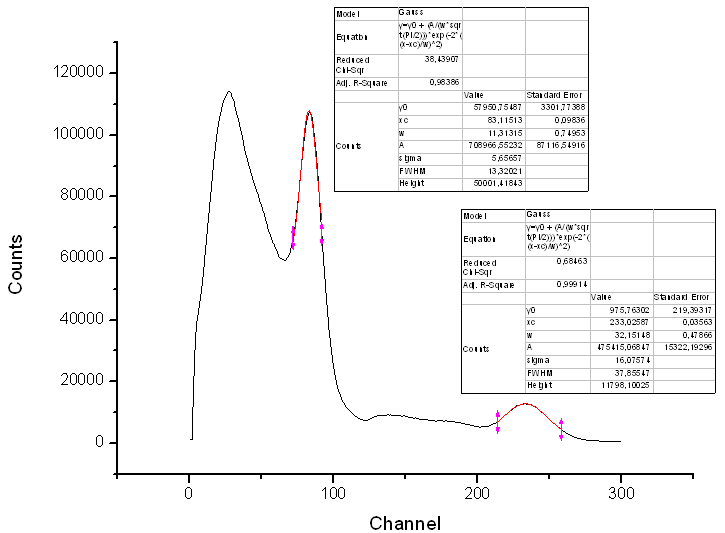
\includegraphics[width=\textwidth]{Graphen/SZ2.png}
 \caption{22Na Spektrum mit SZ2}
\end{figure}

\begin{figure}
 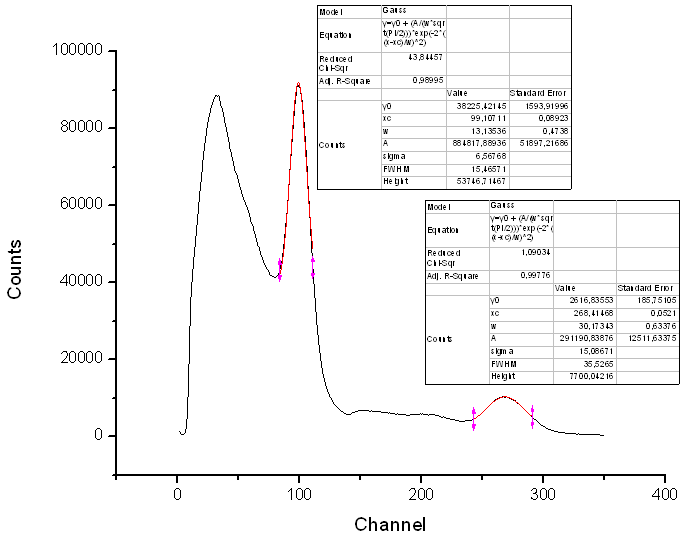
\includegraphics[width=\textwidth]{Graphen/SZ3.png}
 \caption{\Na Spektrum mit SZ3}
\end{figure}  

Dazu haben wir, wie in Abb \ref{schaltplan_sca_lin_mca} dargestellt, das unipolare Signal des Verstärkers (AMP) zur Einstellung des Energiefensters am SCA verwendet. Liegt ein Ereigniss innerhalb dieses Fensters, so wird ein Signal an das Linear Gate gegeben. Dieses lässt dann für einen kurzen Moment das eigentliche (bipolare) Signal durch. Um die Verzögerung durch den SCA (mindestens ca. $0,05\mu s$) kompensieren zu können, wurde zwischen AMP und Linear Gate noch ein Delay eingebaut. Durch die Verzögerungseinstellung des SCA kann jetzt die Laufzeit beider Signale synchronisiert werden. Dazu wurden der positive Normausgang des SCA und der Ausgang des Delays an die Koinzidenz angeschlossen. Über die feinere Verzögerungseinstellung des SCA wurde die Zählrate maximiert. Anschließend wurden beide Signale an das Linear Gate angeschlossen und dessen Ausgangssignal mit dem MCA analysiert. Das genaue Anpassen der Signallaufzeiten ist wichtig, da sonst einerseits zufällige Ereignisse außerhalb des gewünschten Energiefensters gemessen werden, andererseits aber auch das eigentliche Signal abgeschnitten werden kann. Dies würde dann ebenfalls zu einer falschen Energiemessung führen.

Für eine erneute Messung des \Na-Spektrums haben wir folgende Einstellungen verwendet:
\begin{center}
\begin{tabular}{llll}
 & SZ1 & SZ2 & SZ3\\
Verstärkung & 8,12 & 10,0 & 10,0\\
Coarse Gain & 20 & 20 & 20\\
Shaping Time & 0,5 $\mu s$ & 0,5 $\mu s$ & 0,5 $\mu s$\\
Lower Level & 0,04 & 0,04 & 0,0\\
Upper Level & 10,02 & 10,02 & 10,0\\
Delay & 2,14 $\mu s$ & 1,83 $\mu s$ & 2,05 $\mu s$\\
Messdauer & 20 min & 20 min & 20 min\\
Delay SCA & 2 $\mu s$ & 2 $\mu s$ & 2 $\mu s$
\end{tabular}
\end{center}

Aus den Spektren haben wir die Position der 511keV- und 1275keV-Peaks abgelesen: %TODO: gauss-fit? 
\begin{center}
\begin{tabular}{llll}
 & 511keV - Peak (Channel) & 1275 keV-Peak (Channel) \\
SZ1 & $72,4 \pm 0,1$ & $199,2 \pm 0,1$ \\
SZ2 & $83,1 \pm 0,1$ & $233,0 \pm 0,03$ \\
SZ3 & $99,1 \pm 0,1$ & $268,4 \pm 0,1$ 
\end{tabular}
\end{center}

Somit konnten wir eine Energie-Channel-Eichung für die drei Szintillatoren vornehmen:
%TODO: Fehlerrechnung
SZ1: $E = 6,03 keV \cdot c + 74,77 keV$\\
SZ2: $E = 5,10 keV \cdot c + 87,46 keV$\\
SZ3: $E = 4,51 keV \cdot c + 63,79 keV$ \\

\subsection{Zwei-Photonen-Zerfall}

Beim Zerfall des 0S0-Singulett-Zustands des Positroniums können die Photonen, wie in der Theorie näher erläutert, nur in einem $180^\circ$-Winkel abgestrahlt werden. Dies wollen wir über eine Winkelkorrelationsmessung verifizieren. Dazu stellen wir die Szintilatoren auf ein 511keV Fenster ein und drehen SZ1 oder SZ3 gegen den festen SZ2. 

\begin{center}
\begin{tabular}{llll}
 & SZ1 & SZ2 & SZ3\\
Lower Level & 1,585 & 1,87 & 1,79\\
Upper Level & 2,940 & 3,05 & 3,07\\
511keV Peak & 81  & 80 & 94
\end{tabular}
\end{center}

Die Position des 511keV Peaks zeigt also eine Abhängigkeit von der Einstellung der Energiefenster, insbesondere SZ1 mit $\Delta c_{511} = 8,6$. Dies könnte an einer falschen Delay-Einstellung liegen, der wir aber viel Zeit gewidmet haben, an der besseren Filterung durch den SCA oder an Defekten der Elektronik. Wir haben die Fenstereinstellung mit dem MCA und Computer "`auf Sicht"' vorgenommen und denken, dass wir den 511keV-Peak damit hinreichend genau einstellen konnten, auch wenn er nicht mit der vorher vorgenommenen Energieeichung übereinstimmt.

\subsubsection{SZ2 - SZ3}

Wir haben in $180^\circ$-Stellung von SZ2 und SZ3 die Koinzidenzrate mit der Koinzidenzeinheit optimiert. Dazu haben wir die Rate am Hex-Scaler betrachtet und die Delays angepasst.

\begin{center}
\begin{tabular}{llll}
 & Delay\\
SZ2 & 1,83 $\mu s$\\
SZ3 & 2,83 $\mu s$
\end{tabular}
\end{center}

Um den statistische Fehler möglichst klein zu halten (unter 2\%) berechnen wir die nötige Messzeit pro Winkeleinstellung. Bei $150^\circ$ beträgt die Zählrate etwa $n = 3 Hz$, sodass sich die nötige Dauer wie folgt berechnen läßt:
\begin{equation}
 0,02 = \frac{s_N}{N} = \frac{1}{\sqrt{N}} = \frac{1}{\sqrt{n t}} \Leftrightarrow t = \frac{1}{n}\left( \frac{s_N}{N} \right)^{-2} = 833,3s
\end{equation}
Dies entspricht $t \approx 13,89 \text{min}$. Wir wählen daher eine Messzeit von $t = 16,67 \text{min}$ pro Winkeleinstellung, da sich damit die 100Hz-Clock als Stoppsignal für den Hex-Scaler verwenden lässt (100 000 Counts). 

\begin{figure}
 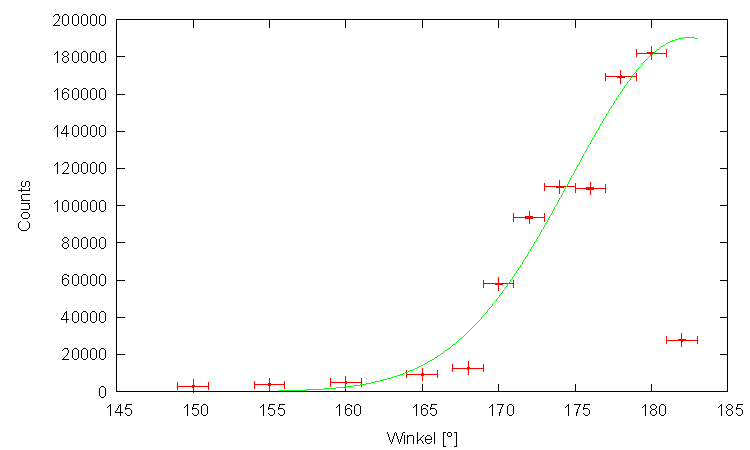
\includegraphics[width=\textwidth]{Graphen/2er/erste.pdf}
 \caption{Winkelkorrelation des Zwei-Photonen-Zerfalls (mit SZ2-SZ3}
\end{figure}


\begin{figure}
 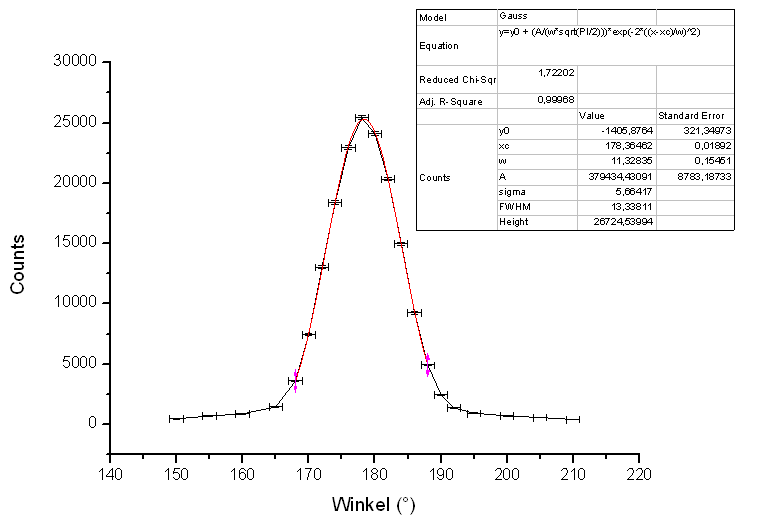
\includegraphics[width=\textwidth]{Graphen/180K.png}
 \caption{Winkelkorrelation des Zwei-Photonen-Zerfalls (mit SZ2-SZ1)}
\end{figure}

\subsection{Drei-Photonen-Zerfall}

\begin{figure}
 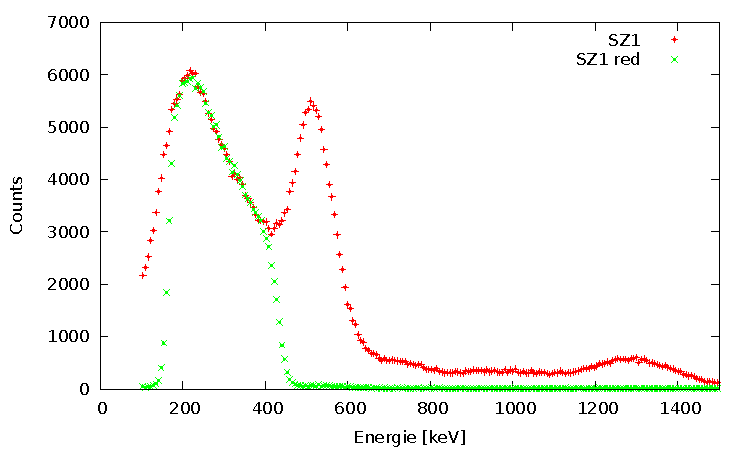
\includegraphics[width=\textwidth]{Graphen/3er/red-spektrum-sz1.pdf}
 \caption{Einstellung des Energiefensters unterhalb der 511keV-Linie für SZ1}
\end{figure}

\begin{figure}
 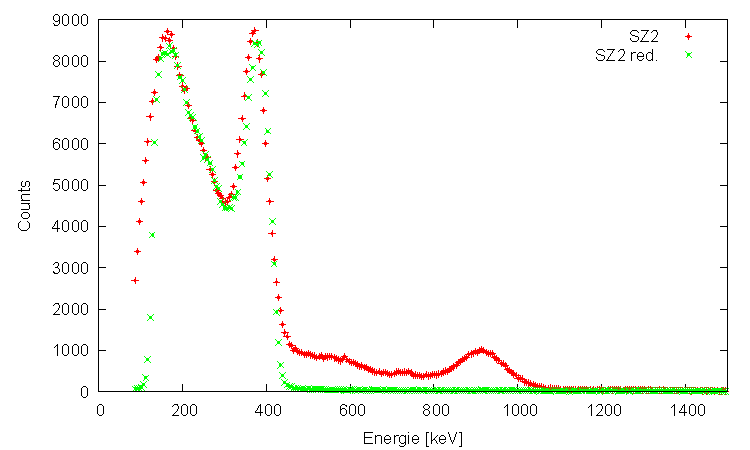
\includegraphics[width=\textwidth]{Graphen/3er/red-spektrum-sz2.pdf}
 \caption{TODO: WAS IST DAS?}
\end{figure}

\begin{figure}
 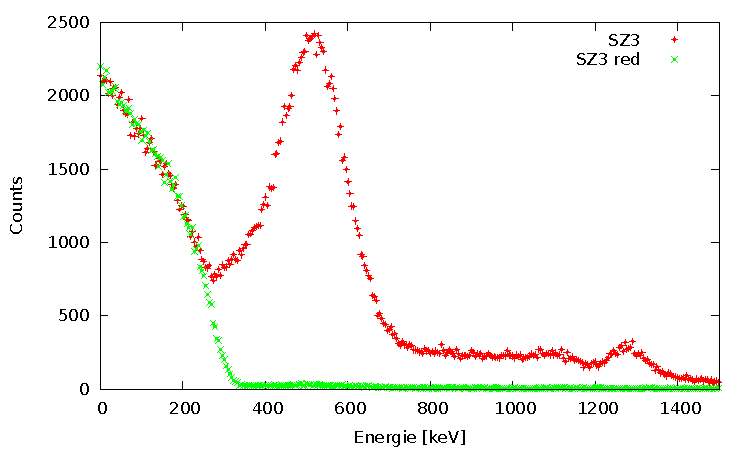
\includegraphics[width=\textwidth]{Graphen/3er/red-spektrum-sz3.pdf}
 \caption{Einstellung des Energiefensters unterhalb der 511keV-Linie für SZ3}
\end{figure}

\begin{figure}
 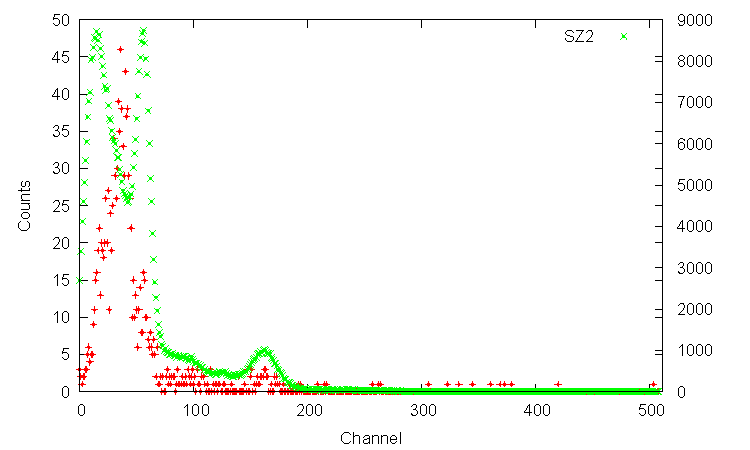
\includegraphics[width=\textwidth]{Graphen/3er/spektrum-1.pdf}
 \caption{Spektrum am SZ2 beim 3er-Koinzidenz}
\end{figure}

\begin{figure}
 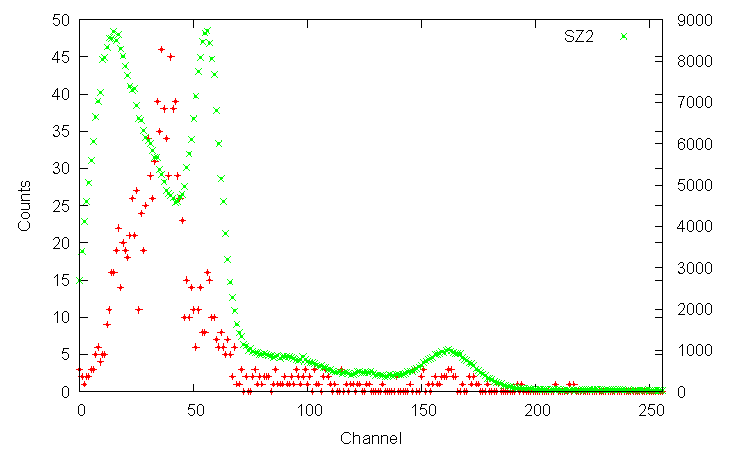
\includegraphics[width=\textwidth]{Graphen/3er/spektrum-2.pdf}
 \caption{Spektrum am SZ2 beim 3er-Koinzidenz}
\end{figure}


\subsection{Quenching}

\begin{figure}
 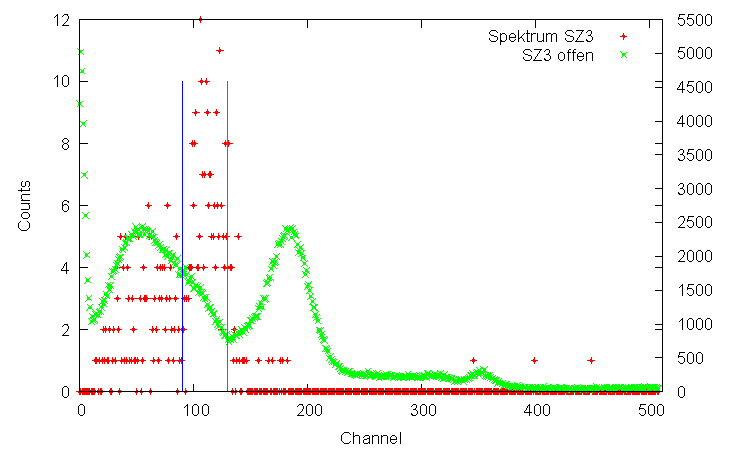
\includegraphics[width=\textwidth]{Graphen/quench/spektrum_0-3.pdf}
 \caption{Spektrum 0,3A}
\end{figure}

\begin{figure}
 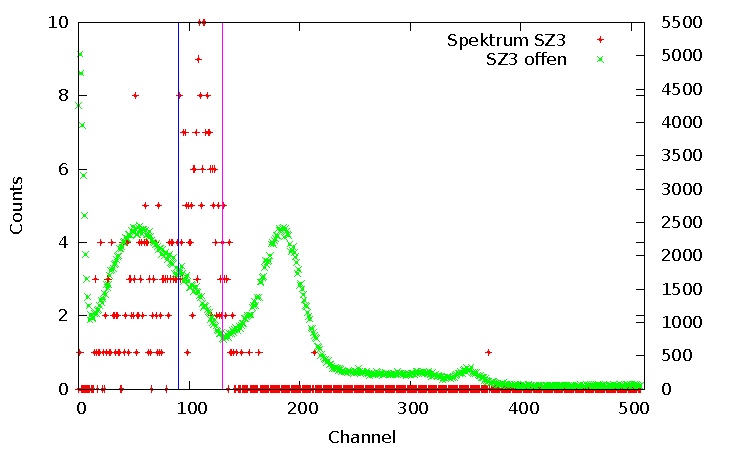
\includegraphics[width=\textwidth]{Graphen/quench/spektrum_1065.pdf}
 \caption{Spektrum 1065G}
\end{figure}


\begin{figure}
 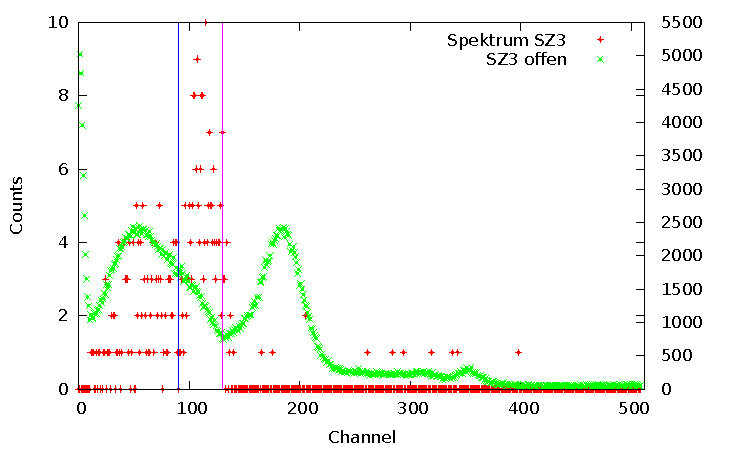
\includegraphics[width=\textwidth]{Graphen/quench/spektrum_2028.pdf}
 \caption{Spektrum 2028G}
\end{figure}


\begin{figure}
 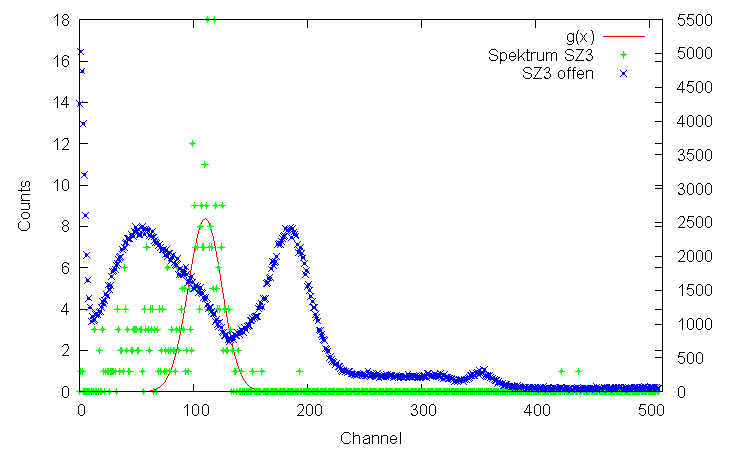
\includegraphics[width=\textwidth]{Graphen/quench/spektrum_0-3_nach_2028.pdf}
 \caption{Spektrum 0,3A nach 2028G}
\end{figure}


\begin{figure}
 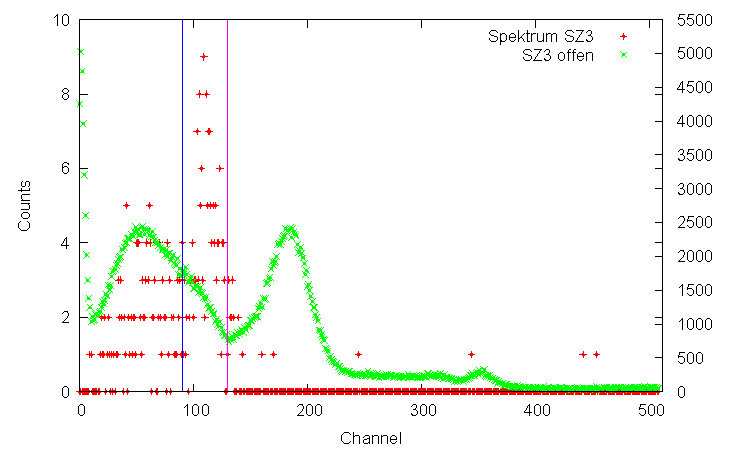
\includegraphics[width=\textwidth]{Graphen/quench/spektrum_3070.pdf}
 \caption{Spektrum 3070G}
\end{figure}

\begin{figure}
 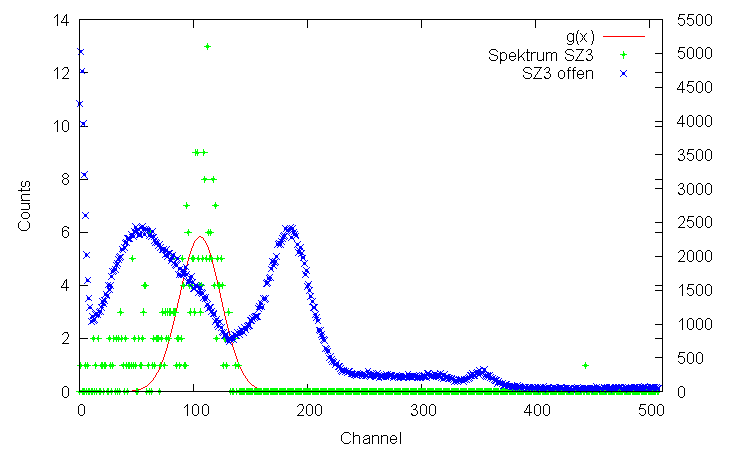
\includegraphics[width=\textwidth]{Graphen/quench/spektrum_4032.pdf}
 \caption{Spektrum 4032G}
\end{figure}

\begin{figure}
 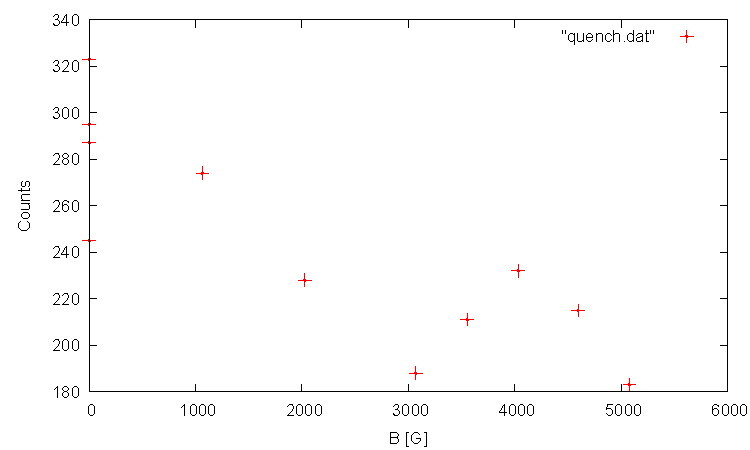
\includegraphics[width=\textwidth]{Auswertung/quench.pdf}
 \caption{Quenching des Drei-Photonen-Zerfalls in $120^\circ$-Konfiguration}
\end{figure}

\begin{figure}
 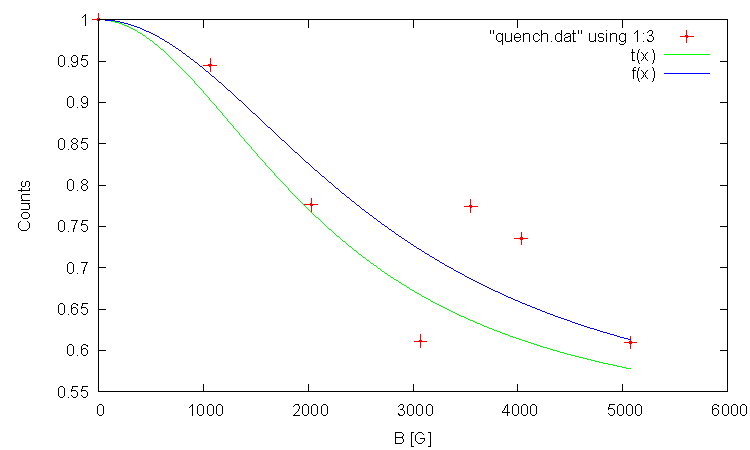
\includegraphics[width=\textwidth]{Auswertung/quench-normiert.pdf}
 \caption{Normiertes Quenching des Drei-Photonen-Zerfalls in $120^\circ$-Konfiguration}
\end{figure}
